\documentclass[jou,apacite]{IEEEtran}
\usepackage{amsfonts}
\usepackage{amsthm}
\usepackage{tabu}
\usepackage{amssymb}
\usepackage{mathtools}
\usepackage{relsize}
\usepackage[font=footnotesize]{subfig}
\usepackage{hyperref}
\usepackage{minted}
\setminted{fontsize=\small, breaklines=true}

\usepackage{graphicx}
\graphicspath{ {../images/} }

\title{A Study in \emph{Scala}bility through Abstraction}

\author{Troy Hu and Benjamin Killeen} % alphabetical by last name

\begin{document}
\maketitle    

\begin{abstract}
  The Scala programming language combines object-oriented and functional
  programming in a single Java-like language intended for mass-adoption. It
  emphasizes component abstraction in a statically typed environment that
  enables remarkably modular software design. In this paper, we provide an
  overview of notable features in the Scala language as well as motivating
  examples that underlie these aspects.\footnote{Source for this paper and its
    examples available at \href{https://github.com/bendkill/scala_project}
    {github.com/bendkill/scala\_project}.}
\end{abstract}                     

\section{Introduction}
\label{sec:intro}

Software components are simply self-contained parts of software used by larger
parts or entire applications. Modern software typically relies on many common
components like hashable types or iterable data structures to use as building
blocks. Component abstraction enables the generalization of implementation for
these features, greatly reducing duplication of effort. It is one of the most
powerful tools in the programmer's utility belt, a fact which the designers of
the Scala programming language aimed to exploit \cite{odersky2004overview}. In
the early 2000s, existing languages had little support for type-sound component
abstraction, including widely used languages like Java and C\#. Odersky \emph{et
  al.} address this shortcoming with a language that combines elements of
object-oriented and functional programming in a statically typed
environment. Scala, which gets its name from ``scalable,'' provides a powerful
interface for abstraction within a development framework intended for mass
adoption.

In pursuit of usability, Scala borrows many syntactic elements from Java and
C\#, and it integrates smoothly with components from these languages. In fact,
the Scala library includes standard Java objects like \texttt{java.lang.String},
as shown in Listing~\ref{lst:print}. Scala code can take advantage of existing
implementations in Java, and in the end it compiles to Java bytecode, making
Scala packages available to Java programmers. At the same time, Scala maintains
a distinct programming paradigm from either Java or C\#. It discards some
features from these languages, and it develops completely novel ideas from the
$\nu$Obj calculus \cite{odersky_nominal_2003}. The example in
Listing~\ref{lst:print} highlights syntactic similarities between Java and Scala,
comparing two implementations of the same program. Note how Java prepends type
declarations before terms, whereas Scala affixes type declarations using the
\texttt{:} operator. This and other changes effect a terser, more expressive
syntax overall.

\begin{listing}
  \centering
  \inputminted[frame=single]{Java}{../examples/PrintExample.java}
  \inputminted[frame=single]{Scala}{../examples/PrintExample.scala}
  \caption{Notice how Scala's general syntax and structure are similar
    to Java's. At the same time, there are some visible differences, e.g., unit
    is returned in the Scala implementation instead of void in the Java
    implementation.}
  \label{lst:print}
\end{listing}

Of course, Scala's foremost strength comes from its typing system. Abstract
class definitions and path-dependent types utilize the $\nu$Obj Calculus,
enabling incredible flexibility through the use of traits and mixins
\cite{odersky_nominal_2003}. Somewhat akin to Java's abstract classes, traits
allow a programmer to rely on abstract methods for common functionalities. For
example, the \texttt{Equiv[T]} trait in Fig.~\ref{lst:equiv} represents an
equivalence relation on the type \texttt{T}, abstracting the definition of
\texttt{eq} on which a concrete method, \texttt{neq} depends. Mixins enable a
class to inherit from multiple traits. For instance, one might use
\texttt{Equiv} in conjunction with an \texttt{Ordering} trait to represent
separate relations on the same type in one object.

Finally, the uniform object model in Scala provides a cohesive programming
environment. Every Scala value is an object, and every operation is a call to a
method. The boolean \texttt{true}, for example, is a singleton object that
extends (inherits from) the Boolean trait (see
Sec.~\ref{sec:traits-obj-cls}). At the same time, Scala fits into a functional
programming paradigm. Functions themselves are values, and the syntax allows for
SML-like decomposition and pattern matching. These features result in a powerful
language with a unified programming experience.

% 3. related work
\section{Related Work}
\label{sec:related-work}

The ideas underlying Scala come from a variety of work. First and foremost, the
designers rely on the $\nu$Obj calculus outlined in Odersky \emph{et al.}
(2003) for a theoretical grounding on which they build Scala's robust type
system \cite{odersky_nominal_2003}. Although a thorough discussion of the
$\nu$Obj calculus is beyond the scope of this paper, which focuses on the Scala
language proper, we describe its main points in brief. Additionally, the ideas
in Scala have been replicated or expanded on in more recent work, which we
discuss here.

The $\nu$Obj calculus is, broadly, a calculus and dependent type system that
includes classes and objects with types as members
\cite{odersky_nominal_2003}. \emph{Dependent types} rely on some value for
definition, and with this formalism, the $\nu$Obj calculus expresses Java's
inner class system, virtual types, and family polymorphism. Furthermore, it
models SML-style modules and functors, diverging from standard object-oriented
type systems in three fundamental ways:
\begin{enumerate}
\item Objects \emph{and} classes are considered primitive, as opposed to just
  objects.
\item Type checking and evaluation rely on name references rather than object
  records.
\item Object types are expressible using possibly nominal type components.
\end{enumerate}
These alterations make possible the rigorous blend of object-oriented and
functional styles evident in Scala, differing markedly from traditional
languages like Java and C\#.

The Rust programming language is a popular alternative to Scala that is designed
to target systems-level applications \cite{matsakis_rust_2014}. The language is
similar to C++ in that it allows users to interact directly with
hardware. Moreover, the syntax of Rust is very similar to that of C++.  Rust,
however, is unlike C++ in that any program purely written in Rust is guaranteed
to avoid memory errors and data races.  Most notably, Rust utilizes many of
Scala's core concepts to achieve its goals.  Like Scala, Rust is both a
functional and object-oriented programming language (to model C++). Rust also
ensures type soundness in order to avoid memory errors such as dangling
pointers. Unlike Scala, however, Rust emphasizes concurrency and paralellism.

The remainder of this paper focuses on the practical considerations of
programming in the Scala language.

\section{Programming in Scala}
\label{sec:programming-scala}

\begin{figure*}[t]
  \centering
  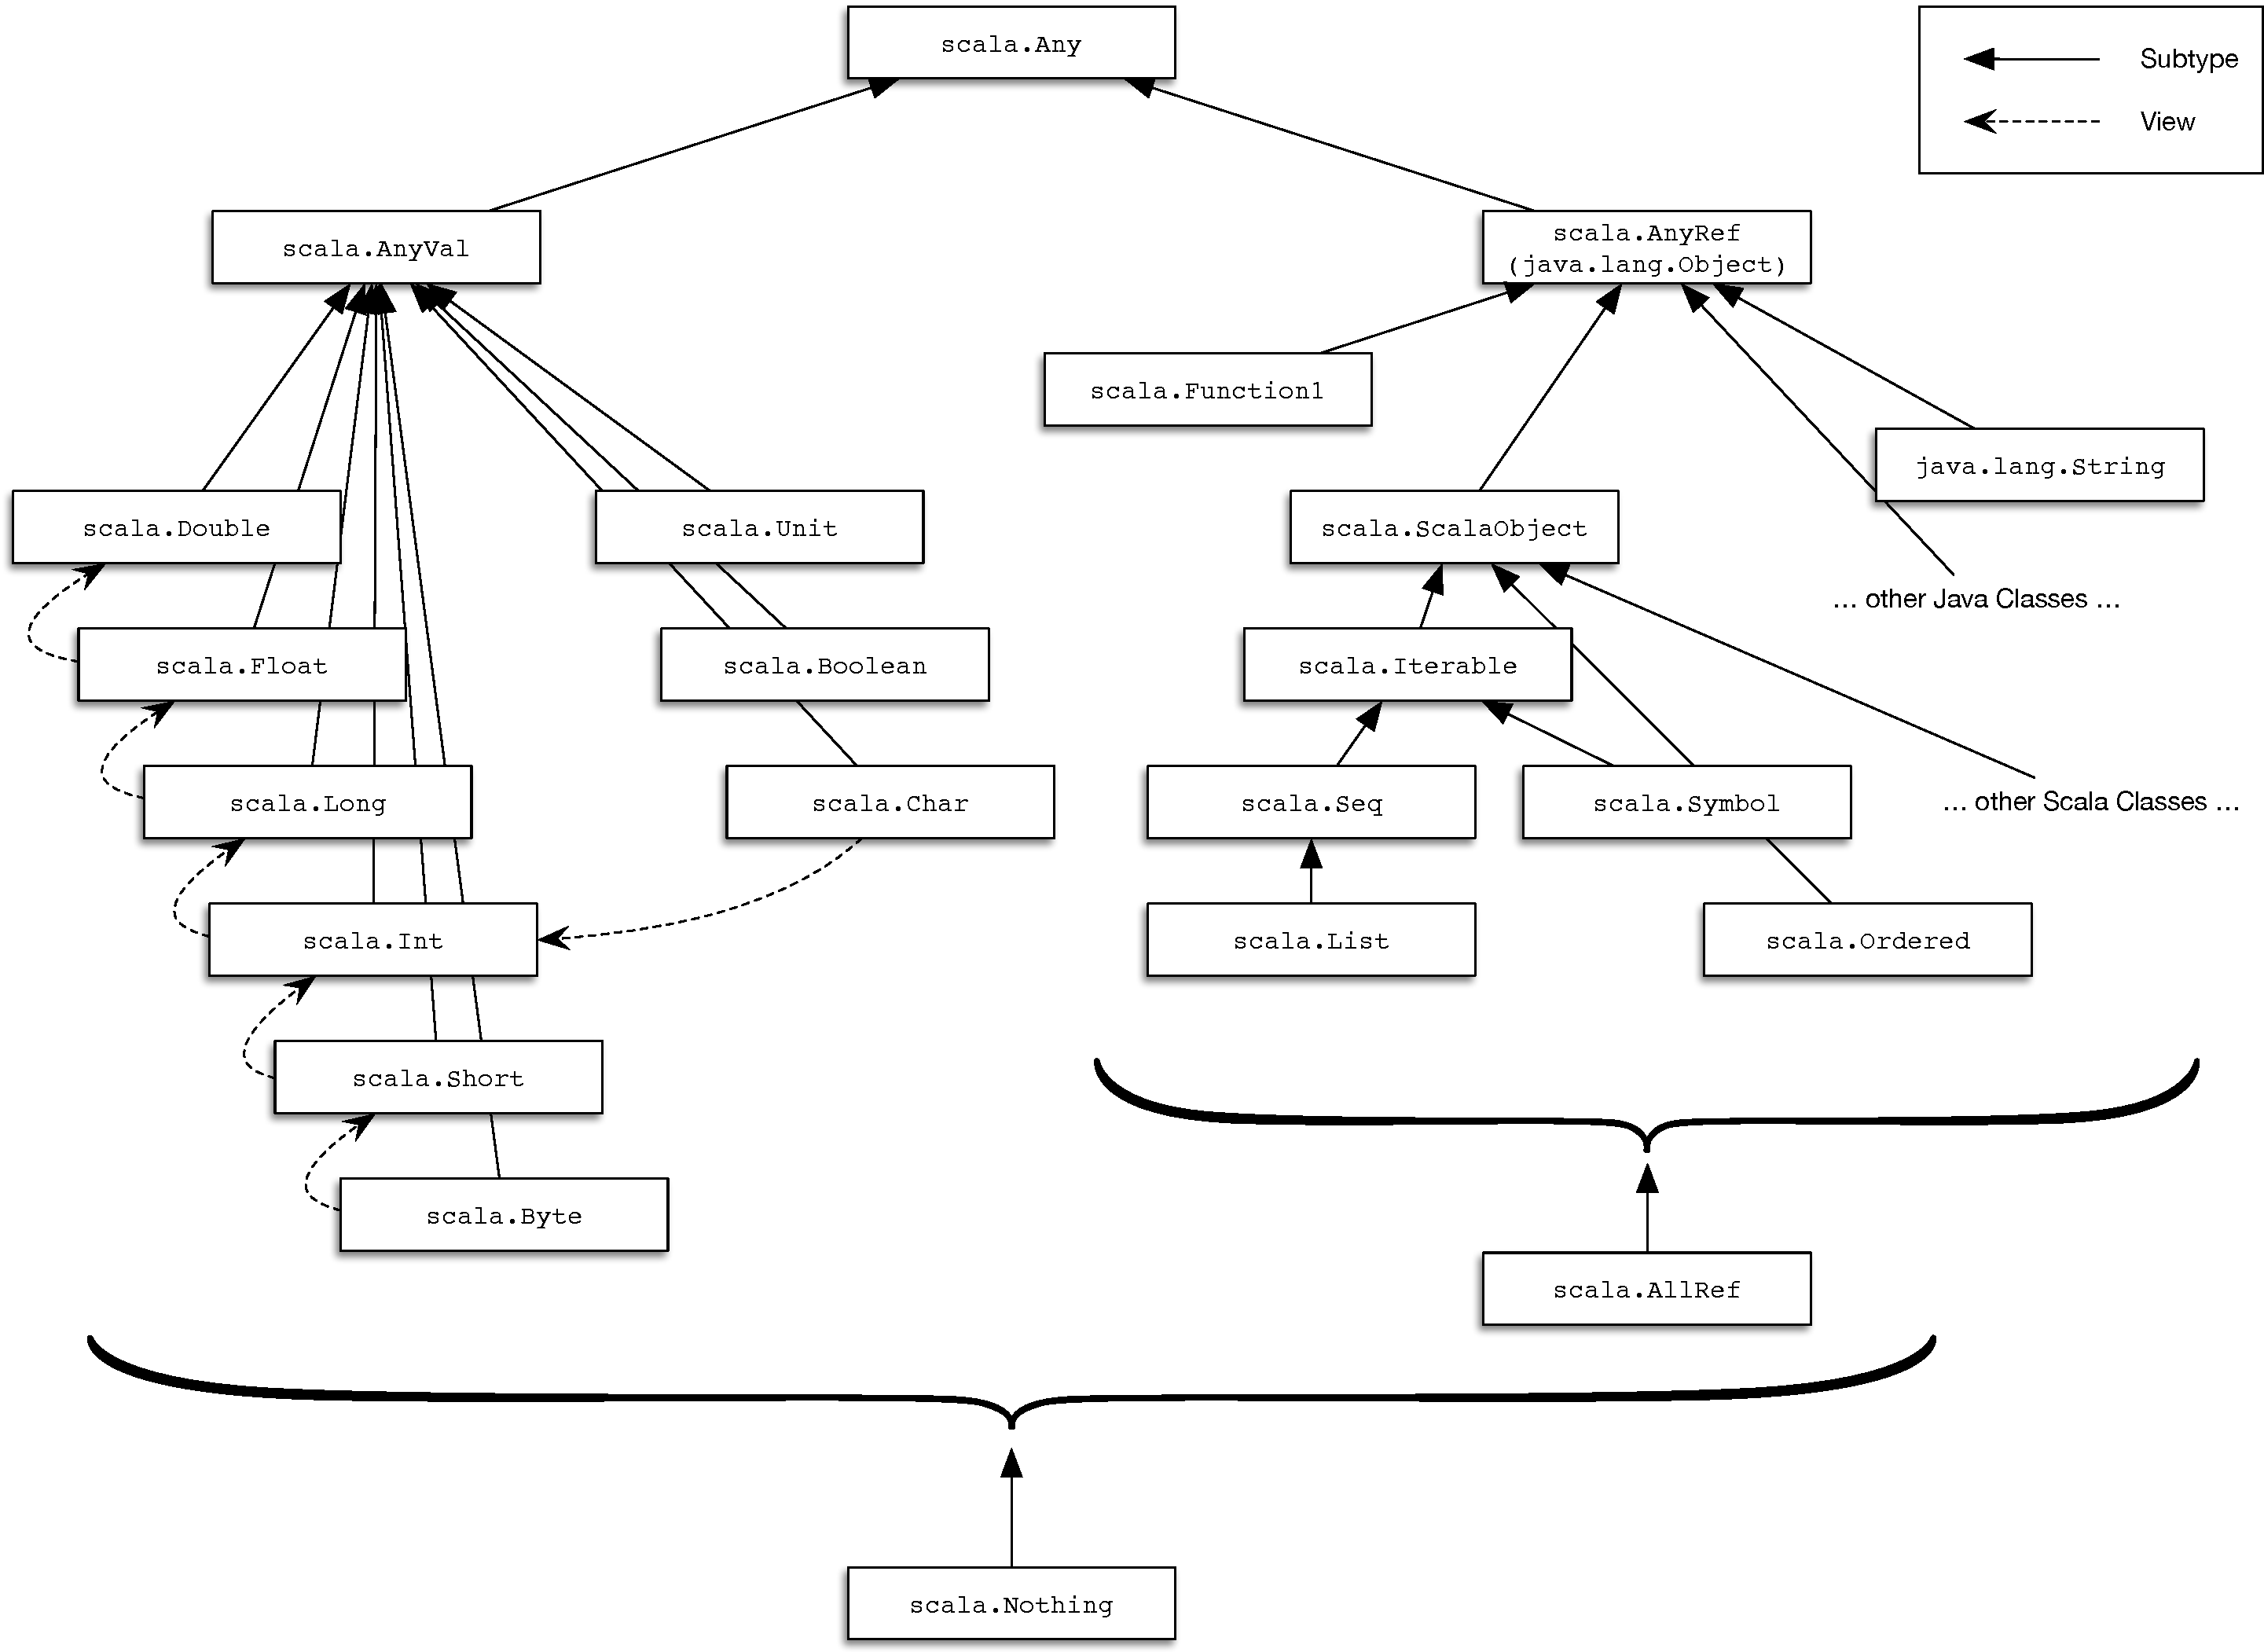
\includegraphics[width=0.9\linewidth]{scala_classes}
  \caption{A visual representation of Scala's class hierarchy}
  \label{fig:scala-classes}
\end{figure*} 

Being a fully developed programming language, Scala implements numerous useful
features that encourage modularity and reusability in software. In this section,
we highlight just a few of these, as well as provide an overview of the general
process through which software construction takes place in Scala.

\subsection{Unified Object Model}
\label{sec:unified-object-model}

In Scala, every value is an object and every class is a subtype of the
\texttt{Any} class. Fig.~\ref{fig:scala-classes} shows an overview of the
unified object model in Scala's standard library, under which many classes
simply absorb the existing Java implementation. Immutable objects or
\emph{values}, denoted with the \texttt{val} keyword on declaration, inherit
from the class \texttt{AnyVal}, and include classes like \texttt{scala.Boolean}
and \texttt{scala.Char}. Mutable \emph{variables} on the other hand, inherit
from \texttt{scala.AnyRef}, which is synonymous with the generic
\texttt{java.lang.Object}. These include classes like \texttt{scala.List} or
traits like \texttt{scala.Ordered}. Even functions fit into this object model,
such as the \texttt{scala.Function1} trait, which single-argument functions
implement.

One of the fundamental aspects of Scala is its invariance with respect to value
representation. Under this rule, \emph{interpreting an value belonging to some
  subclass as an element of its superclass does not change that value's
  representation.} Put another way, this invariance rule demands that for types
\texttt{S}, \texttt{T} with \texttt{S~<:~T}, and \texttt{x} of type \texttt{S},
\begin{minted}{Scala}
x.asInstanceOf[T].asInstanceOf[S] = x
\end{minted}
always holds. Because of this rule, Scala's object model includes some unusual
relations not found in more traditional languages. In particular,
Fig.~\ref{fig:scala-classes} uses dashed lines to denote a \emph{View} from one
type to another. As discussed in Sec.~\ref{sec:views}, a view enables
interpretation between types which are not strictly subtypes of one another. For
example, both \texttt{Int} and \texttt{Float} maintain a member called
\texttt{MaxValue}, which other function can rely on without requiring a strict
subtype of either \texttt{Int} or \texttt{Float}. Finally, the
\texttt{scala.Nothing} trait is a subtype of every other class, allowing for
flexible objects like the \texttt{scala.List} object \texttt{Nil}, of type
\texttt{List[Nothing]}.

Another fundamental feature of Scala's object model inclusion of operations,
which are invocations of a method. For example, the usual addition operator
\texttt{+} can be implemented like any other method, as in
Lst.~\ref{lst:nat-full}, and invoked in the exact same way: \texttt{x.+(y)}.  Of
course Scala allows for the more conventional calling style \texttt{x + y}, but
it does so merely through syntactic sugaring. Here, \texttt{x} is the receiver
object, \texttt{+} is a method defined in \texttt{x}, and \texttt{y} is the
method's argument.

Finally, Scala differs from Java with regard to the construction of
objects. Rather than define a dedicated constructor function within objects, the
class name itself is simply the constructor. Object instantiations simply runs
the entire body of the class, instantiated member variables, values, and
definitions.

\subsection{Traits, Objects, and Classes}
\label{sec:traits-obj-cls}

Traits in Scala are somewhat akin to abstract classes in Java, defining abstract
members that should be implemented by more concrete classes. As a very simple
example, consider the \texttt{Nat} trait which defines necessary operations on
natural numbers: %
\begin{samepage}
  \inputminted{Scala}{../examples/ExampleNat.scala} %
\end{samepage}

Classes which inherit from \texttt{Nat} must implement the \texttt{isZero},
\texttt{succ}, and \texttt{pred} methods with the corresponding types in order
to inherit from \texttt{Nat}. This is advantageous for several reasons. First,
as we shall see, the \texttt{Nat} class may use these abstract methods to define
more complex functions, which subclasses need not implement. Second, other
functions may refer to \texttt{Nat}s as a whole rather than either subclass of
the original trait.

Objects or singleton objects in Scala often accompany trait definitions. A
singleton object is at the same time a class definition and the sole
instantiated member of that class. For instance, the \texttt{Z} object
represents the natural number ``zero,'' of which there can only be one: %
\begin{samepage}
  \inputminted{Scala}{../examples/ExampleZero.scala} %
\end{samepage}
This simple implementation behaves as we would expect, relying on the \texttt{S}
class (below) to implement \texttt{Z.succ}. The choice to ensure \texttt{Z.pred
  = Z} was made in keeping with conventional evaluation rules. The use of the
\texttt{extends} keyword represents the inheritance from \texttt{Nat}.

Similarly classes in Scala can ``extend'' a trait, while taking in arguments to
the constructor. The \texttt{S} class %
\begin{samepage}
  \inputminted{Scala}{../examples/ExampleSucc.scala} %
\end{samepage}
represents the ``successor'' of another natural \texttt{n}, either \texttt{Z} or
another \texttt{S}. Here, the use of the \texttt{case} keyword results in a
constructor very similar to constructors in SML, which can be instantiated
without the use of \texttt{new} and easily deconstructed in pattern matching
blocks.

\subsection{Views}
\label{sec:views}

In place of loose subtyping, Scala requires views to implicitly convert objects
from one type to another. A view is implemented with a method that takes in an
arguemnt of one type and returns an object of another type. The only difference
between a view method and a normal method is that view methods require the
\texttt{implicit} modifier, which goes before the method definition. This
modifier allows the Scala compiler to know that it is the implcit conversion
method when converting from one type to another. Scala implictly applies a view
to an expression, $e$ of type $T$, when one of the following cases occur:
\begin{itemize}
\item The expected type of $e$ is not of type $T$.
\item A member selected from $e$ is not a member of $T$.
\end{itemize}  
For example, in Lst.~\ref{lst:set-example}, \texttt{listToSet} is the view that
converts \texttt{GenList[T]} to \texttt{Set[T]}. The compiler inserts
applications of the view onto \texttt{xs}.

\begin{listing}
  \inputminted[frame=single, firstline=3, lastline=14]{Scala}{../examples/Set.scala}
  \caption{An example of views and implcit conversions.}
  \label{lst:set-example}
\end{listing}

\subsection{Type Parameters}
\label{sec:type-parameters}

Scala's focus on component abstraction would not be complete without the
inclusion of type parameters or variables. These allow a function or class to be
implemented without a specific type in mind while remaining type sound. As a
simple example, consider the identity function $f(x) = x$ which has type
$\tau \rightarrow \tau$. This cannot be constrained to any particular type
\texttt{Int} or \texttt{Boolean} without fundamentally changing its
behavior. Fortunately, Scala allows for this flexibility with type variables:
\begin{minted}{Scala}
def identity [T] (x: T): T = x
\end{minted}
In this definition, \texttt{[T]} designates a type without constraints which the
argument \texttt{x} belongs to, as well as the return type of the function, also
\texttt{T}. Since the body of function simply returns $x$ without invoking any
methods or assuming any properties, this is valid.

Scala traits can also rely on type parameters in much the same
way. Lst.~\ref{lst:equiv} shows a very simple trait that defines equivalence
relations on arbitrary types, as long as an implementation of \texttt{eq} exists
on that type. Not that one must distinguish between a type that can be compared
for equality and an equality relation on some type. \texttt{Equiv[T]} represents
the latter. Lst.~\ref{lst:ordering} shows a similar trait that describes
an ordering on some type \texttt{T}, which we use to implement ordered lists in
the abstract.

\begin{listing}
  \inputminted[firstline=3, frame=single]{Scala}{../examples/Equiv.scala} 
  \caption{An abstraction of equivalence relations in Scala.}
  \label{lst:equiv}
\end{listing}

\begin{listing}
  \inputminted[firstline=3, frame=single]{Scala}{../examples/Ord.scala}
  \caption{An abstraction of ordering relations in Scala.}
  \label{lst:ordering}
\end{listing}

Scala also allows for constraints on type parameters. These include the subtype,
supertype, and view relations: \texttt{<:}, \texttt{>:}, and \texttt{<\%}
respectively. These can be used in concert with one another, as in the following
method for lexicographic comparison of lists:
\begin{minted}{Scala}
trait LexList[+T] {
  // ...standard list methods...
  def < [U >: T <: Ordered[U]](that: LexList[U]): Boolean = {
    !that.isEmpty && 
    (this.isEmpty ||
     this.head < that.head || 
     this.head == that.head ||
     this.tail < that.tail)
  }
}
\end{minted}
In \texttt{LexList.<}, \texttt{that} must contain elements that are supertypes
of the elements of \texttt{this}, since \texttt{U >: T}. Moreover, both elements
must inherit from the standard \texttt{Ordered[T]} trait, since \texttt{U <:
  Ordered[U]}. This makes possible the calls to \texttt{<} and \texttt{==}. View
relations are used similarly, where \texttt{U <\% T} requires that an implicit
view exists to convert objects of type \texttt{U} to type
\texttt{T}.

Crucially, Scala includes strict enforcement of the variance of these types. A
type constructor \texttt{C} is \emph{covariant} if for \texttt{A <: B},
\texttt{C[A] <: C[B]}. Similarly, \texttt{C} is \emph{contravariant} if
\texttt{C[A] >: C[B]} and invariant if neither relation can be guaranteed. Type
parameters are declared invariant by default and covariant or contravariant
using the \texttt{+} or \texttt{-} prefixes respectively. In the
\texttt{LexList} example as well as Lst.~\ref{lst:ordlist-full}, we declare the
type constructor to be covariant, as lists should be. Scala enforces this
declaration at compile time by ensuring that \texttt{T} is used in covariant
positions throughout the body of the trait.

This enforcement is commonly a source of some confusion. The \texttt{OrdList[T]}
from Lst.~\ref{lst:ordlist-full} has an \texttt{insert} method, for instance,
that takes an argument \texttt{x: U} where \texttt{U >: T}. Intuitively, one
would think that \texttt{x: T} should be sufficient, but in fact this is not
possible in order for \texttt{OrdList} to be covariant. Consider the bad
definition:
\begin{minted}{Scala}
// bad typing for insert! 
trait OrdList[+T] {
  def insert(x: T, o: Ordering[T]): OrdList[T];
}
\end{minted}
and suppose we had \texttt{Integer} in addition to \texttt{Nat}, both with a
common supertype \texttt{Number}. Since \texttt{Nat <: Number} and
\texttt{Integer <: Number}, covariance requires that
\begin{minted}{Scala}
OrdList[Nat] <: OrdList[Number]
\end{minted}
and
\begin{minted}{Scala}
OrdList[Integer] <: OrdList[Number]
\end{minted}
Suppose \texttt{insert} accepted \texttt{x: T} for \texttt{OrdList[T]}. Then an
\texttt{OrdList[Nat]} could not insert an \texttt{Integer}, a fact which causes
the following function to fail:
\begin{minted}{Scala}
def pushNumber (x: Number, 
                l: OrdList[Number], 
                o: Ordering[Number]): 
    OrdList[Number] = l.insert(x, o)
\end{minted}
Under subtyping, \texttt{push} accepts an \texttt{x: Integer} and \texttt{l:
  OrdList[Nat]}, but with these arguments, the call to \texttt{insert} will
fail. Under the proper type definition, however, inserting \texttt{x} into
\texttt{l} will result in an \texttt{OrdList} of their common supertype,
\texttt{Number}. This is proper covariance.

\subsection{Mixins}
\label{sec:mixins}

Scala allows for multiple inheritance through the use of mixins. These address
the diamond inheritance problem, which refers to possible ambiguities that arise
from multiple inheritance. Every class inherits methods primarily through the
first superclass listed, allowing for a single path of superclass
dependencies. This disambiguates collisions of class members, as in
Lst.~\ref{lst:mixin}, which implements the usual ordering on $\mathbb{N}$ by
defining \texttt{leq} as well as an equivalence relation that compares the
evenness of two naturals, through \texttt{equal}. The collision here occurs
between \texttt{Ordering[T]}'s \texttt{neq}, which depends on \texttt{leq}, and
\texttt{Equiv[T]}'s \texttt{neq}, which depends on \texttt{equal}. Because
\texttt{NatOrderingWithEquiv} extends first from \texttt{Ordering[Nat]}, it will
use the definition that depends on \texttt{leq}.

\begin{listing}
\inputminted[frame=single, firstline=5]{Scala}{../examples/MixinExample.scala}
\caption{A single object representing two relations on Naturals, an ordering and
an equivalence relation.}
\label{lst:mixin}
\end{listing}

\begin{listing*}[p]
  \inputminted[frame=single, fontsize=\scriptsize, linenos=true]
  {Scala}{../examples/Nat.scala}
  \caption{Complete implementation of the \texttt{nat} package.}
  \label{lst:nat-full}
\end{listing*}

\begin{listing*}[p]
  \inputminted[frame=single, fontsize=\scriptsize, linenos=true]
  {Scala}{../examples/OrdList.scala}
  \caption{Complete implementation of the \texttt{ordlist} package, which
    requires an \texttt{Ordering[T]}. Note how \texttt{OrdList[T]} is covariant,
    so \texttt{insert} requires argument \texttt{x} to be of a supertype of
    \texttt{T}.}
  \label{lst:ordlist-full}
\end{listing*}

% 4. report on peano arithmetic calculator.
\section{Application: Peano Arithmetic Calculator}
\label{sec:appl-peano-arithm}

Although this paper includes significant engagement with the Scala language
merely to describe its features, we consider illustrative examples a poor
indicator of a language's friendliness toward component abstraction. In order to
truly evaluate Scala's scalability, we implement a full-scale interpreter for a
small calculator language called \texttt{peano}. The full description of this
language is beyond the scope of this paper, but it includes sufficient
complexity to take full advantage of Scala's flexibility. \texttt{peano} gets
its name from the Peano Arithmetic, with which all expressions are evaluated
\cite{grassmann_lehrbuch_1861}. The \texttt{peano} interpreter is implemented in
a mostly functional style with separate objects \texttt{Scanner},
\texttt{Parser}, \texttt{Desugarer}, \texttt{TypeChecker}, and
\texttt{Evaluator} that interpret \texttt{peano} expressions. It includes the
standard operations on naturals, integers, and rationals: addition,
multiplication, \emph{etc.}, while also providing higher level functions like
GCD and LCM. These challenges gave us the opportunity to work with Scala in the
same setting that large-scale developers do, using its built-in project manager
\texttt{sbt}.

In general, we found Scala to be simple to work with. Scala development is vast
improvement over existing workflows in Java and C\#, even without taking
advantage of component abstraction, due to the language's more expressive
syntax. It's error messages are informative, and the built-in package manager
\texttt{sbt} takes care of the many nuances of software construction and
deployment. The scope of \texttt{peano}, initially envisioned as a much simpler
calculator language that used built-in numeric types for evaluation, attests to
our enjoyment of programming in Scala.

The source for \texttt{peano} as well as basic usage instructions can be found at
\href{https://www.github.com/bendkill/peano}{github.com/bendkill/peano}.

% 5. should encapsulate discussion of current status
\section{Discussion}
\label{sec:discussion}

After 15 years, Scala has been regularly updated and is currently at stable
release version 2.12.8. Over this period, the core principles of Scala have
remained the same. Scala has achieved widespread adoption in the industry with
companies such as Twitter and Apple utilizing the language. Moreover, Scala has
both a large academic and non-academic user base. The language is often cited or
used in computer science research. In addition, Scala's user community is
thriving. There exist chatrooms, subreddits, and research conferences devoted
entirely to Scala. The community maintains up-to-date documentation and
installation instructions at \href{https://www.scala-lang.org/}{scala-lang.org}.


\bibliographystyle{IEEEtran}
\bibliography{scala_project}

\end{document}

%%% Local Variables:
%%% mode: latex
%%% TeX-master: t
%%% TeX-command-extra-options: "-shell-escape"
%%% End:
